% Original vector figures. Dimensions are controlled; figure text stays at 9 pt.
\tikzset{mfxbox/.style={draw=black!70,fill=black!3,rounded corners=1pt,align=center,inner sep=4pt,minimum height=9mm},mfxarrow/.style={-{Stealth[length=1.8mm]},line width=.65pt},mfxcontrol/.style={mfxarrow,dashed},mfxlabel/.style={font=\fontsize{9}{10.5}\selectfont,align=center,fill=white,inner sep=2pt},mfxgroup/.style={draw=black!40,rounded corners=2pt,inner sep=5mm}}
\newcommand{\MFXArchitectureDiagram}{%
\begin{tikzpicture}[font=\fontsize{9}{10.5}\selectfont,x=1cm,y=1cm]
\node[mfxbox,text width=15mm] (guitar) at (0,0) {Guitar};
\node[mfxbox,text width=30mm] (input) at (3.9,0) {MCP6002\\conditioner};
\node[mfxbox,text width=29mm] (dsp) at (8.7,0) {TSA1701\\ADC / DSP / DAC};
\node[mfxbox,text width=22mm] (amp) at (12.2,0) {PAM8302\\module};
\node[mfxbox,text width=14mm] (speaker) at (15,0) {Speaker};
\node[mfxbox,text width=20mm] (uart) at (2.7,-1.75) {CP2102N\\USB--UART};
\node[mfxbox,text width=20mm] (mcu) at (5.2,-1.75) {STM32F030\\buttons / LEDs};
\node[mfxlabel] (usb) at (0,-1.75) {PC / USB};
\draw[mfxarrow] (guitar)--(input);\draw[mfxarrow] (input)--(dsp);
\draw[mfxarrow] (dsp)--(amp);\draw[mfxarrow] (amp)--(speaker);
\draw[mfxcontrol] (usb)--(uart);\draw[mfxcontrol] (uart)--(mcu);
\draw[mfxcontrol] (mcu.east)--(8.7,-1.75)--node[mfxlabel,right]{I\textsuperscript{2}C}(dsp.south);
\begin{scope}[on background layer]\node[mfxgroup,inner sep=3mm,fit=(input)(uart)(mcu)] (pcb) {};\end{scope}
\node[mfxlabel,anchor=north west] at (pcb.south west) {Custom PCB: 5 V distribution and 3.3 V control};
\node[mfxlabel,anchor=north] at (11.4,-2.3) {External audio modules and speaker};
\end{tikzpicture}}

\newcommand{\MFXInputCircuitDiagram}{%
\begin{circuitikz}[font=\fontsize{9}{10.5}\selectfont]
\node[op amp] (b) at (7.4,0) {U2B};
\draw (.7,0 |- b.+) node[ocirc,label=left:{J2 TIP}]{} to[C,l=C7,a=470 nF] (2.1,0 |- b.+)
 to[R,l=R5,a=4.7 k$\Omega$] (4.3,0 |- b.+) -- (b.+);
\draw (4.9,0 |- b.+) node[circ]{} to[R] (4.9,-2.7);
\node[mfxlabel,anchor=east,align=right] at (4.55,-1.6) {R6 + R7 + R8\\1.006 M$\Omega$};
\node[mfxlabel,anchor=north] at (4.9,-2.8) {VREF\_AUDIO};
\draw (.7,-1.1) node[ocirc,label=left:{J2 SLEEVE}]{} -- (.7,-1.65) node[ground]{};
\draw (b.-) -| (6,1.55) to[R,l=R9,a=10 k$\Omega$] (9.3,1.55) -- (9.3,0) -- (b.out);
\draw (6,1.55) -- (6,2.65) to[nos,l=JP3] (9.3,2.65) -- (9.3,1.55);
\draw (6,1.55) to[R,l_=R10,a^=10 k$\Omega$] (3.5,1.55) node[anchor=east]{VREF\_AUDIO};
\draw (9.3,0) to[R,l=R11,a=100 $\Omega$] (11.2,0) to[C,l=C8,a=1 $\mu$F] (13.3,0) -- (14.5,0) node[ocirc,label=above:{to JP7.1}]{};
\draw (14,0) node[circ]{} to[R,l_=R12,a^=226 k$\Omega$] (14,-2.45) node[ground]{};
\node[mfxlabel] at (8,-1.85) {U2: MCP6002-I/P\\Supply: +5V\_A / GND};
\node[op amp] (a) at (4.4,-4.6) {U2A};
\draw (.5,-3.25) node[anchor=south]{+5V\_A} to[R,l=R3,a=10 k$\Omega$] (.5,-5.09)
 to[R,l=R4,a=10 k$\Omega$] (.5,-6.85) node[ground]{};
\draw (.5,0 |- a.+) node[circ]{} -- (a.+);
\draw (2.1,0 |- a.+) node[circ]{} to[C,l=C6] (2.1,-6.85) node[ground]{};
\draw (a.out) -- (6.7,-4.6) node[ocirc]{} node[anchor=south]{VREF\_AUDIO};
\draw (a.-) -- ++(-.25,0) |- (4,-3.25) -| (5.95,-4.6) node[circ]{};
\node[mfxlabel,align=left,text width=66mm] at (10.8,-5.7) {C6 = 10 $\mu$F filters the divider.\\C5 = 100 nF decouples U2 locally.\\The buffered reference is distinct from system ground.};
\end{circuitikz}}

\newcommand{\MFXResponsePlots}{%
\begin{tikzpicture}
\begin{semilogxaxis}[width=8.25cm,height=6.3cm,xlabel={Frequency (Hz)},ylabel={Source-to-module gain (dB)},xmin=.1,xmax=20000,ymin=-45,ymax=9,grid=both,minor grid style={gray!10},major grid style={gray!25},label style={font=\fontsize{9}{10}\selectfont},tick label style={font=\footnotesize},legend style={font=\footnotesize,at={(.03,.97)},anchor=north west,draw=none,fill=white},legend cell align=left]
\addplot[black,thick] table[x=frequency,y=gain_one_db,col sep=comma]{response.csv};\addlegendentry{JP3 closed: gain 1}
\addplot[gray,thick] table[x=frequency,y=gain_two_db,col sep=comma]{response.csv};\addlegendentry{JP3 open: gain 2}
\addplot[gray,dashed] table[x=frequency,y=gain_two_low_db,col sep=comma]{response.csv};
\addplot[gray,dashed] table[x=frequency,y=gain_two_high_db,col sep=comma]{response.csv};
\end{semilogxaxis}
\begin{axis}[at={(8.45cm,0)},anchor=south west,width=8.1cm,height=6.3cm,xlabel={Analog rail $V_A$ (V)},ylabel={Guitar sine input (V RMS)},xmin=3,xmax=5.25,ymin=0,ymax=2,grid=major,major grid style={gray!25},label style={font=\fontsize{9}{10}\selectfont},tick label style={font=\footnotesize},legend style={font=\footnotesize,at={(.03,.97)},anchor=north west,draw=none},legend cell align=left]
\addplot[black,thick,domain=3:5.25,samples=30]{(x/2-\MFXHeadroomMarginV)/(sqrt(2)*10^(\MFXInputAttenuationDb/20))};\addlegendentry{Nominal gain 1}
\addplot[gray,thick,domain=3:5.25,samples=30]{(x/2-\MFXHeadroomMarginV)/(2*sqrt(2)*10^(\MFXInputAttenuationDb/20))};\addlegendentry{Nominal gain 2}
\node[font=\footnotesize,align=center,anchor=south] at (rel axis cs:.5,.03) {Illustrative reserve: \MFXHeadroomMarginV\ V\\Centered reference; not a swing guarantee};
\end{axis}
\end{tikzpicture}}

\newcommand{\MFXPcbLayoutDiagram}{%
\begin{tikzpicture}[font=\fontsize{9}{10.5}\selectfont]
\node[inner sep=0] (pcbimage) {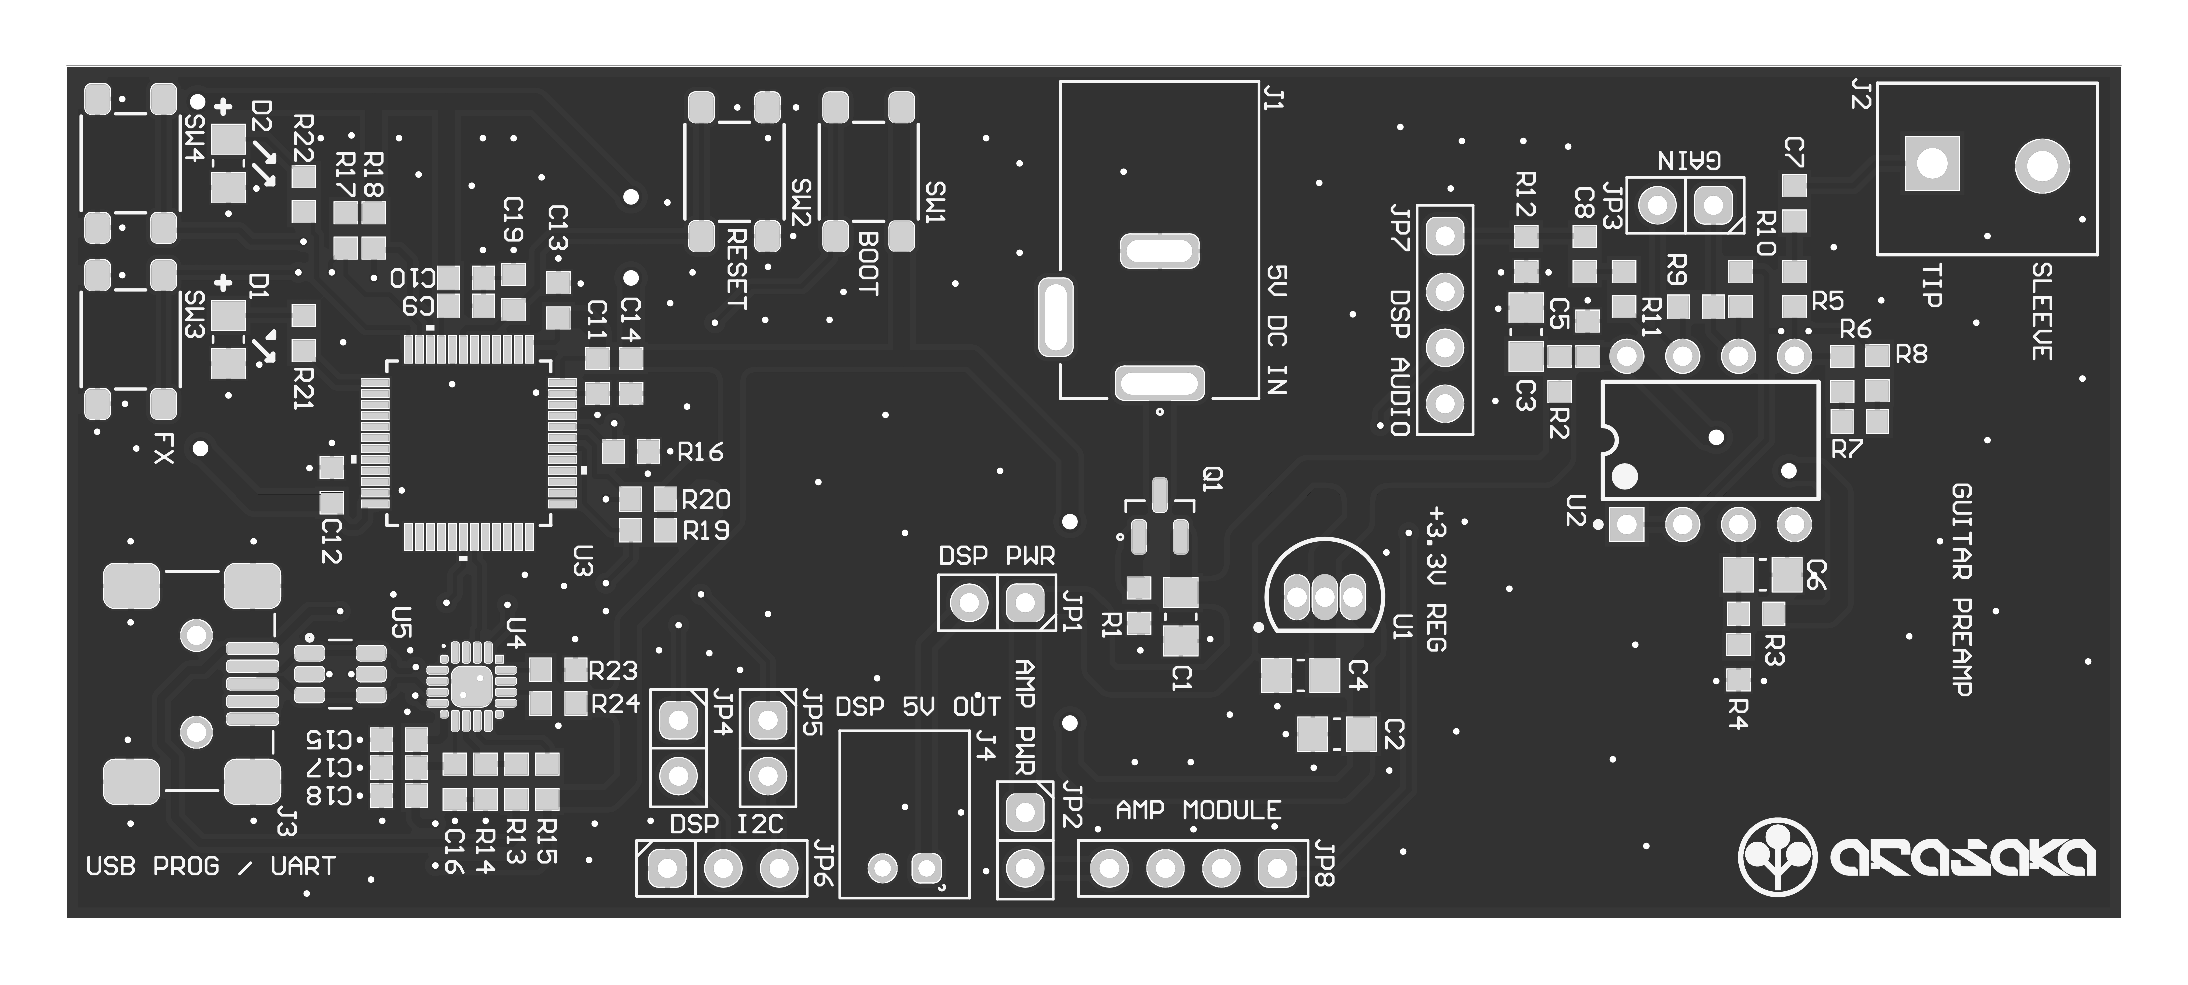
\includegraphics[width=.96\linewidth]{figures/pcb-top.pdf}};
\node[mfxlabel,above=6mm of pcbimage.north west,anchor=south west] (left) {Controller / USB\\Local digital decoupling};
\node[mfxlabel,above=6mm of pcbimage.north] (middle) {5 V entry / regulation\\Supply branches and returns};
\node[mfxlabel,above=6mm of pcbimage.north east,anchor=south east] (right) {Guitar input / U2\\Short, high-impedance path};
\draw[mfxarrow] (left.south)--($(pcbimage.north west)!.22!(pcbimage.north east)+(0,-15mm)$);
\draw[mfxarrow] (middle.south)--($(pcbimage.north west)!.52!(pcbimage.north east)+(0,-20mm)$);
\draw[mfxarrow] (right.south)--($(pcbimage.north west)!.86!(pcbimage.north east)+(0,-10mm)$);
\node[mfxlabel,below=5mm of pcbimage.south] {Inspect both copper layers and cable returns. Regions alone do not prove isolation.};
\end{tikzpicture}}

\newcommand{\MFXConnectionsDiagram}{%
\begin{tikzpicture}[font=\fontsize{9}{10.5}\selectfont,x=1cm,y=1cm]
\node[mfxbox,text width=55mm,minimum height=52mm] (board) at (3.1,0) {};
\node[anchor=north,font=\bfseries\fontsize{9}{10.5}\selectfont] at (3.1,2.35) {Main PCB};
\node[mfxlabel,anchor=west,align=left] at (.65,1.4) {JP7.1: conditioned audio\\JP7.2 / .4: GND\\JP7.3: DSP line return};
\node[mfxlabel,anchor=west,align=left] at (.65,.05) {JP6.1: GND\\JP6.2: SCL / JP6.3: SDA\\JP4 / JP5: MCU isolation};
\node[mfxlabel,anchor=west,align=left] at (.65,-1.5) {J4.1: +5V\_TSA / J4.2: GND\\JP8.1: line / JP8.2--3: GND\\JP8.4: +5V\_AMP};
\node[mfxbox,text width=32mm,minimum height=23mm] (dsp) at (10.2,1.2) {TSA1701\\ADC0 / DAC0 / GND\\SCL / SDA / GND};
\node[mfxbox,text width=32mm] (amp) at (10.2,-2) {PAM8302 module\\Input / GND / 5 V};
\node[mfxbox,text width=18mm] (spk) at (14.5,-2) {Speaker\\OUT+ / OUT$-$};
\node[mfxlabel] (usbi) at (14.5,1.2) {USBi\\3.3 V logic / GND};
\draw[mfxarrow] (5.85,1.8)--node[mfxlabel,above]{audio input}(8.35,1.8);
\draw[mfxarrow] (8.35,1.2)--node[mfxlabel,below]{line return}(5.85,1.2);
\draw[mfxcontrol] (5.85,.2)--(7,.2)--(7,.6)--(8.35,.6);
\draw[mfxcontrol] (usbi.west)--(dsp.east);
\draw[mfxarrow] (5.85,-1.2)--(7.6,-1.2)--(7.6,-2)--(amp.west);
\draw[mfxarrow] (amp.east)--(spk.west);
\node[mfxlabel,align=left,anchor=north west] at (0,-3.05) {Normal: verify JP1/JP2 power branches before closing. USBi service: JP4/JP5 open, JP2 open.\\J4 powers TSA1701 through microUSB; USBi's separate 5 V output stays disconnected.\\Verify the physical module header order; these numbers belong to the main PCB only.};
\end{tikzpicture}}

\newcommand{\MFXTestSetupDiagram}{%
\begin{tikzpicture}[font=\fontsize{9}{10.5}\selectfont,x=1cm,y=1cm]
\node[mfxbox,text width=26mm] (gen) at (1,0) {Signal generator\\Known source / level};
\node[mfxbox,text width=34mm] (dut) at (6,0) {PCB + TSA1701\\Known unity DSP route};
\node[mfxbox,text width=28mm] (amp) at (11,0) {Amplifier\\Connect last};
\node[mfxbox,text width=19mm] (load) at (14.6,0) {Resistive load\\Known rating};
\draw[mfxarrow] (gen)--(dut);\draw[mfxarrow] (dut)--(amp);\draw[mfxarrow] (amp)--(load);
\node[mfxbox,text width=34mm] (scope) at (6,-2) {Scope / audio acquisition\\Input, bias and line output};
\node[mfxbox,text width=28mm] (diff) at (12.5,-2) {Differential acquisition\\Filtered BTL output};
\draw[mfxcontrol] (dut)--(scope);\draw[mfxcontrol] (load.south)|-(diff.east);
\node[mfxlabel] at (1,-2) {Current-limited 5 V\\DMM / current readout};
\node[mfxlabel,anchor=north] at (8,-3) {Record supply, load, signal, bandwidth, configuration and ambient for every result.};
\end{tikzpicture}}
